\documentclass[11pt,a4paper,twoside,titlepage,british]{report}
\setlength{\topmargin}{18pt}
\usepackage{layout}
\usepackage[utf8]{inputenc}         % special chars
\usepackage[babel]{csquotes}        % context-sensitive quotation
\usepackage[dvipsnames]{xcolor}     % some predefined colors
\usepackage[plain]{fancyref}        % provides \fref and \Fref for referencing
\usepackage[T1]{fontenc}
\usepackage{babel}
\usepackage{isodate}
\usepackage{fancyhdr}
\usepackage{geometry}
\usepackage{hyperref}
\usepackage[style=numeric-comp,sorting=none,backend=biber]{biblatex}
\usepackage{graphicx}
\usepackage{setspace}
\usepackage{amsmath}
\usepackage{float}
\usepackage{listings}

\geometry{
    textheight=595pt,
    textwidth=360pt,
}

\addbibresource{main.bib}
\nocite{*}

%=======================================================================================================================

\fancyhf{}
\fancyfoot[LE,RO]{\thepage}
\fancyhead[LE,RO]{\slshape \nouppercase{\leftmark}}
\renewcommand*{\headrulewidth}{0pt}
\renewcommand*{\footrulewidth}{0pt}
\fancypagestyle{plain}{%
  \fancyhf{}
  \fancyfoot[LE,RO]{\thepage}
}
\renewcommand*{\chaptermark}[1]{\markboth{\thechapter.\ #1}{}}
\renewcommand*{\sectionmark}[1]{\markright{\thesection.\ #1}}

%=======================================================================================================================

\author{Lukas Wilde}
\date{31.08.2022}
\title{Workload-based Data Partitioning for Index Construction}

%=======================================================================================================================

\makeatletter
\let\runauthor\@author
\let\runtitle\@title
\let\rundate\@date
\makeatother
\sloppy

%=======================================================================================================================

\begin{document}
\pagenumbering{roman}
\begin{titlepage}
    \begin{center}
        
\includegraphics[scale=.5]{figures/logo.pdf}

        \bfseries
        \vspace{2em}
        Faculty of Natural Sciences and Technology I \\
        Department of Computer Science

        \vspace{2cm}
        \begin{doublespace}
            {\LARGE \runtitle}
        \end{doublespace}

        \vspace{1cm} 
        {\large Bachelor's Thesis}

        \vfill
        {\normalfont written by}
        \\[1em]
        {\Large \runauthor}
        \\[1em]
        \textbf{\printdate{\rundate}}

        \vfill
        {\normalfont Supervisors}
        \\
        {\large Jens~Dittrich}
        \\[.5em]
        {\normalfont Advisor}
        \\
        {\large First Advisor}
        \\[.5em]
        {\normalfont 1st Reviewer}
        \\
        {\large Jens~Dittrich}
        \\[.5em]
        {\normalfont 2nd Reviewer}
        \\
        {\large Second Reviewer}
    \end{center}
\end{titlepage}
\setcounter{page}{2}

%=======================================================================================================================

\cleardoublepage
\thispagestyle{plain}
\vspace*{\fill}

\subsection*{Eidesstattliche Erklärung}
Ich erkläre hiermit an Eides Statt, dass ich die vorliegende Arbeit selbstständig verfasst und keine anderen als die
angegebenen Quellen und Hilfsmittel verwendet habe.

\subsection*{Statement in Lieu of an Oath}
I hereby confirm that I have written this thesis on my own and that I have not used any other media or materials than
the ones referred to in this thesis.

\vspace{2cm}

\subsection*{Einverständniserklärung}
Ich bin damit einverstanden, dass meine (bestandene) Arbeit in beiden Versionen in die Bibliothek der Informatik
aufgenommen und damit veröffentlicht wird.

\subsection*{Declaration of Consent}
I agree to make both versions of my thesis (with a passing grade) acessible to the public by having them added to the
library of the Computer Science Department.

\vspace{2.5cm}

\begin{tabular}{ c c c c }
    Saarbrücken, & \makebox[4cm]{\hrulefill} & & \makebox[4cm]{\hrulefill} \\ [-2.2mm] 
               & \tiny Datum/Date                &              & \tiny Unterschrift/Signature \\
\end{tabular}

\vspace*{\fill}


%=======================================================================================================================

\thispagestyle{plain}
\chapter*{Acknowledgement}

\clearpage
\thispagestyle{plain}

\chapter*{Abstract}


%=======================================================================================================================

\cleardoublepage
\thispagestyle{plain}
\setcounter{tocdepth}{1} % do not print subsections
\setcounter{tocdepth}{2} % but add them to the PDF
\tableofcontents

%=======================================================================================================================

\cleardoublepage
\pagenumbering{arabic}
\chapter{Introduction}

Here is a citation \cite{btree}.
\begin{itemize}
    \item DBMS routinely use index structures for increased performance
    \item Index pre-configured or chosen by user
    \item Mostly no utilization of underlying data or workload distribution
    \item Except: learned indexes -> Related Work
    \item Motivation: different data structures for different query workloads (hash table?)
    \item For this, introduce concept of hybrid index structures
    \item Create partitions to create singular indexes and combine them
    \item Optimize partitions based on one/multiple metrics
    \item As motivation: GENE, starting point for generic search
    \item Introduce what is covered in what section of this thesis
\end{itemize}

%=======================================================================================================================

\clearpage
\thispagestyle{plain}
\chapter{Related Work}\label{sec:related_work}

This chapter covers work related to Workload-based Data Partitioning. I also introduce the index structures used as baselines in the evaluation.

The well-known B$^+$-tree \cite{Bayer1970-rh} is the first basic index structure used in the comparison.

The second index used for comparison is the Adaptive Radix Tree (ART) \cite{Leis2013}. The authors recognize that the B$^+$-tree is widely used for disk-based database systems but indicate that it is unsuitable for modern-day main-memory databases. This is mainly due to the disparity of CPU cache sizes and main memory speed making main memory access times no longer uniform. Also, there is the problem of CPU stalls, which is caused by the CPU being unable to predict the result of comparisons easily. As comparisons are necessary to  traverse a B$^+$-tree, this causes more latency for the index. To overcome these problems, the authors introduce an improvement to Radix Trees, which uses certain parts of the keys directly to guide the search in the tree. While Radix Trees get rid of the afore-mentioned CPU stalls, they often have to make a global trade-off between tree height and space efficiency. This problem is solved by introducing adaptive nodes with varying capacities to hold child pointers. Results show that ART can outperform other main-memory data structures, with the only competitor being a hash table. As these store keys in a random order, they cannot support range queries efficiently and are only useful in specific scenarios.

To cover the last index structure used in the comparison, we need to look at another class of index structures that only emerged recently. Learned index structures generally try to leverage recent progress in the field of Machine Learning to improve index performance.

The Recursive Model Index (RMI) \cite{Kraska2018} introduces the concept that indexes are models that simply map keys to positions in a sorted array. The authors state that most modern index structures do not consider the data distribution and miss out on highly relevant optimizations. While most datasets don't follow simple patterns, they argue that Machine Learning approaches can be used to incorporate these patterns. One can look at traversing a B$^+$-tree as slowly reducing the error it takes to find the final location of the key (e.g.~ 100M possible records are reduced to 1M). The same approach can be adapted to Machine Learning models. While it is hard to guarantee that a single model will reduce the error from 100M (possible keys) to hundreds for the final search, it is reasonable for a model to do so from 100M to 10k. With this in mind, the authors construct a hierarchy of Machine Learning models, where each model picks the next layer's model that should be used to predict the position of the key. This hierarchy does not need to follow a strict tree structure; each model can cover an individual number of keys. The benefit of this architecture lies in the ability to customize the models. For example, the bottom layer of nodes could only represent linear regression models (as there are many leaves and linear regression models are quite inexpensive), while higher up, one could use more complex neural network structures. The data segmentation happens through the given structure and training of the internal node's models. While this paper introduces the use of the underlying data distribution for index construction, it suffers from the explainability of neural networks. Therefore, there are no clear properties that could be used for my work.

FITing-Tree \cite{Galakatos2019} tries to combine the flexibility of traditional index structures with learning by indexing linear data segments. The data partitioning is done by a single pass over the sorted data. The segmentation algorithm aims to determine the data segments' bounds so that the relation between keys and positions in the sorted array can be approximated by a linear function. To give reliable performance estimates, an error parameter is used to indicate how much an estimated position is allowed to deviate from the real position. A new segment is created once a point falls outside an error cone that ensures this maximum deviation. Otherwise, the cone is adjusted by tightening its bounds. Once the segments are determined, they are indexed by a B$^+$-tree to find a key's corresponding segment, and a binary search is performed inside the segment to find the actual position of the key.

The authors of the Piecewise Geometric Model index (PGM) \cite{Ferragina:2020pgm}, which I used as the third baseline in the evaluation, tried to improve upon the ideas of FITing-Tree. While FITing-Tree's approach seemed reasonable, a disadvantage was the data segmentation. The authors note that the single-pass segmentation algorithm does not produce the optimal number of data segments, leading to more data segments, a larger tree height, and increased lookup time. By reducing the segmentation to the problem of constructing a convex hull and allowing the index to be built recursively, they could increase the lookup time and ensure provably efficient time and space bounds in the worst case.

TODO: Distribution-aware PGM

While learned index structures perform so well because they can adapt to the underlying data distribution, apart from the distribution-aware PGM, they do not consider the workload that will be executed. RMI partition the data indirectly through their models, FITing-Tree and PGM explicitly use segmentation algorithms before building the index to determine the data that belongs in one segment. However, workload information might be beneficial to index construction, e.g.~by indicating that certain data segments are not frequently requested. My work covers this problem: can workload information be used to improve data segmentation and thereby yield better performance?

Adaptive Hybrid Indexes \cite{Anneser2022} tackle the problem of selecting suitable encodings inside index structures to trade-off between space utilization and index performance. Compact indexes reduce the index's memory, allowing the database system to utilize that free memory to accelerate queries. However, they are naturally inferior to performance-optimized indexes. The decision of what encoding should be used on which part of the index is hard to make at build-time. Therefore, the authors propose to make these decisions at run-time. They introduce a framework that allows for monitoring the accesses across the index nodes when queries are processed, and based on these metrics, they classify whether nodes are cold or hot. Using so-called context-sensitive heuristic functions (CSHF), the framework determines, based on the classification of hot- and coldness, the memory budget, the historical classifications, and other properties, whether a node should have a compressed or performance-optimized encoding. Especially relevant to my work is the classification as hot or cold. Once the data is split into segments and inserted into a tree-like structure, it could be beneficial to modify the index based on this classification. While the authors do this at run-time, my work focuses on analyzing the workload before building the index. They use encodings for this, but one could also consider shifting leaves in the tree higher up to optimize for cache benefits.

    \begin{itemize}
    \item GENE \cite{Dittrich2021} for the approach to look at indexes as logical components and combining them, generic
    search briefly to iterate over starting options and give our partitioning as a possible better starting point.
    \end{itemize}

Distributed database systems are another field where the workload is used for partitioning. An example there is Schism \cite{Curino2010}. The motivation behind this approach is to improve the performance and scalability of distributed databases. Each tuple is represented as a node in a graph. Two nodes are connected if the corresponding tuples occur in the same transaction. The edges are weighted with the total amount of co-occurrences in transactions. Given a number of partitions $k$, the algorithm will find a set of cuts of the edges that produces $k$ distinct partitions with roughly equal weight and minimal costs along the cut edges. The intuition behind this is that tuples that are often accessed in the same transaction should also reside in the same partition/node to optimize query processing. By minimizing the cost along the cut edges, pairs of tuples that are seldom accessed together are split into different partitions, whereas often connected tuples stay in the same partition. While I don't look at transaction-based workloads in this work, there is a similarity in looking at workload properties to partition the data. Schism uses the frequency of co-occurrences to do this partitioning, which indicates that the frequency of query accesses could be a promising property to look at.

\clearpage
\thispagestyle{plain}
\chapter{Background}

\section{Hybrid Index Structures}
\begin{itemize}
    \item What are hybrid index structures?
    \item Advantages: optimize for subproblems, combine to one index
    \item challenges: correct combination of these structures (e.g.~routing through data structure)
\end{itemize}

\section{Partition and Partitioning functions}
\begin{itemize}
    \item Mathematical set theory definition of partition
    \item Adaption to key space/segments
    \item Partitioning functions for indexes
    \item Used in routing of through index
\end{itemize}

\section{Numerical Differentiation}
\begin{itemize}
    \item Finite difference approximations
    \item Relation to true derivative (limes h -> 0)
    \item Consistency order of approximations
    \item Forward, Central, Backward finite difference approximations
\end{itemize}



\clearpage
\thispagestyle{plain}
\chapter{Framework}
This chapter introduces the framework that was implemented to generate workloads, partition data and eventually benchmark a custom index that uses the partitioning. Note that the terms partitions and segments will be used interchangeably in the following.
\begin{figure}[H]
    \centering
    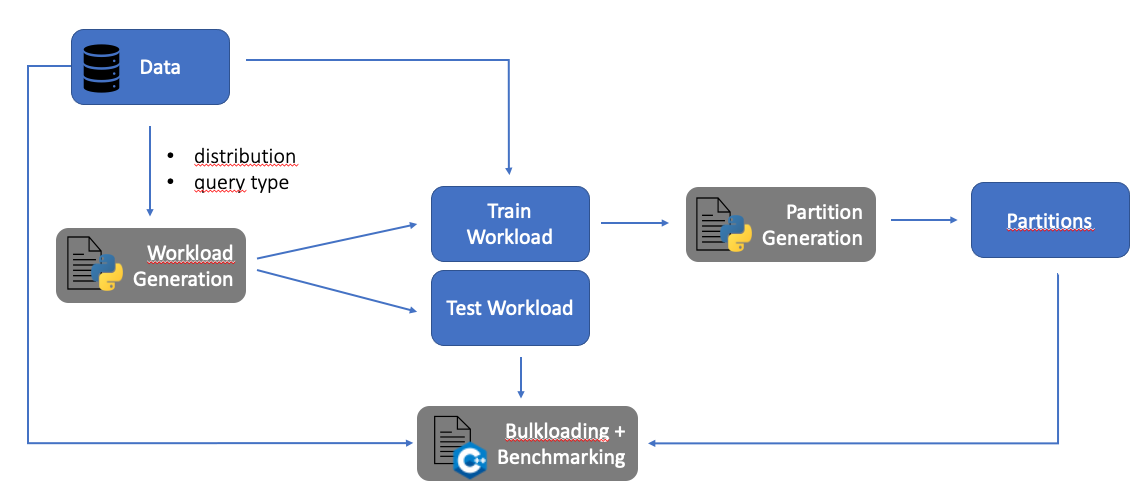
\includegraphics[width=\textwidth]{figures/pipeline.png}
    \caption{Framework Overview}
    \label{fig:framework}
\end{figure}

\section{Overview}
As we can see in Figure \ref{fig:framework}, the origin of all processes is the underlying data that should be indexed. Using a python script, we can specify properties like the distribution and type of queries (point, range) that should be generated to access the data through the index. The queries generated by this step are divided into a train and test workload and saved to files for later use in the C++ benchmarking.

TODO: Example of overlapping distributions

Given the train workload, the partitioning algorithms that are described in Sections \ref{sec:frequency} and \ref{sec:purity} can analyze the corresponding properties of the workload and will produce a partition of the underlying data. The resulting elements are saved to a file with additional information that can be used for the index construction.
With this partition, the index is bulkloaded from the data where each element of the partition corresponds to an individual leaf node. The additional information like relative frequency and predominant query type of a segment can be used to modify the index. For example, if only point queries access a segment, it could be beneficial to manage data access through a hash table instead of a normal B-tree leaf. The next step is to execute the test workload on the index and compare it to other state-of-the-art indexes that were introduced in Section \ref{sec:related_work}, namely a B$^+$-tree, an Adaptive Radix Tree (ART) and a Piecewise Geometric Model index (PGM).

\section{Workload Generation}
The ultimate goal of this work is to generate good partitions for the index construction like it was mentioned in Section \ref{bg:hybrid}. The inputs to the partitioning algorithms are therefore a dataset and a workload sample which we know is representative of the expected workload. However, for the purpose of evaluating and testing the algorithms and modifications later used, we were in need of a flexible way to generate workload data, especially since it proved hard to find available real-world workload data. The workload generation is done in a Python script specifying a series of \verb|Region| objects that wrap the following information:

\begin{itemize}
    \item \verb|qtype|: The query type that should be generated in this section, e.g.~point or range queries
    \item \verb|num|: The number of queries for this section
    \item \verb|distribution|: Distribution underlying the generated queries, e.g.~normal, uniform, ...
    \item \verb|index|: Whether the generation happens index-based or domain-based
    \item \verb|min, max|: minimal and maximal values that indicate the section boundaries. Either index or domain-based, depending on the value of \verb|index|.
\end{itemize}

This gives us a very flexible way to generate arbitrary workloads. Note that while a partition generated for the index construction later satisfies that the elements are mutually disjoint, the \verb|Region| objects used for workload generation do not need to be disjoint. This only means that we can overlap the boundaries of the objects to generate even more flexible workloads. In fact, it is the only way to generate regions of the data that are accessed through multiple types of queries, e.g.~ through both point and range queries. 

\section{Partitioning algorithms}
There are a plethora of properties that one could look at when analyzing query workloads, but inspired by the works in Section \ref{sec:related_work}, we decided to focus on two properties and look at how we could use these to partition the data and create segments. As described in the previous Section, we can use the train workload to partition the data. The test workload is immediately saved to file after creation and not seen by both partitioning algorithms. 

\subsection{Partitioning by Frequency} \label{sec:frequency}
The first algorithm analyzes the frequency of query access for each key in the key space. The motivation behind using the frequency as partition property is that hopefully we can benefit from caching effects during execution of the test workload. We would hope that highly frequent segments remain in cache so that subsequent queries can retrieve the location of the corresponding keys faster. Additionally, by analyzing the frequency, we can use that information to change the structure of the index. A first idea in this regard would be to shift highly frequent segments higher up in the tree, to prevent expensive pointer chasing when traversing the index.

We first realized, that key-by-key comparisons are not useful for a generalized partitioning algorithm because we can only operate on a train workload that is sampled from the general workload distribution. If we would use these key-by-key comparisons for the frequency to create partitions, we would probably overfit to the patterns in the train workload, even though these might only be caused by noise and not be present in the general distribution. Therefore, we employ an approach that tries to maximize the previously mentioned goal: find partitions where keys are accessed roughly the same amount of times. This partition should create elements, that utilize caching. Regions with almost no accesses will be put in one partition which will result in the segment being not loaded very often. On the other hand, regions with similarly frequent keys will result in the the corresponding segment remaining in cache if the frequency is high enough.

We use a single-pass algorithm that tries to find plateaus in the workload distribution by calculating the average change in frequency over a sliding window. It uses three phases depending on where it currently is with respect to a plateau, which are heavily inspired by the finite difference approximations from Section \ref{bg:numerical}:

\begin{enumerate}
    \item Start calculating a discrete forward difference approximation. As only keys "in the future" are considered, this phase is predestined to find an incoming plateau by checking if the calculated slope is near 0.
    \item After such a plateau was found, we use the central difference approximation to establish the boundaries of the plateau. We use this approximation now, as it considers keys from before and after the current one. This should give a better estimation of when a plateau is ending.
    \item Once the central approximation indicates that a plateau is ending, we switch to calculating the backward finite difference approximation to ensure that we find the exact end point of the plateau. We only consider previous keys, as we now know that an end is coming and this gives us the best chance to catch the key that is responsible for significantly changing the slope.
\end{enumerate}



\begin{algorithm}
\caption{Partition by Frequency}
\begin{algorithmic} 
    \STATE $idx \leftarrow 0$
    \STATE $n \leftarrow data.size$
    \WHILE{$idx < n - w$}
    \STATE $current\_freq \leftarrow freq[idx]$
    \STATE $fwd\_mean \leftarrow mean(freq[idx : idx + w])$
    \STATE $fwd\_slope \leftarrow fwd\_mean / w$
    \IF{$isclose(fwd\_slope, 0, delta / w)$}
    \STATE $potential\_start \leftarrow idx$
    \STATE $idx \leftarrow idx + 1$
    \FOR{$i \text{ in } 1 .. w // 2$}
    \STATE $central\_left \leftarrow mean(freq[idx - i : idx + 1])$
    \STATE $central\_right \leftarrow mean(freq[idx + 1 : idx + w // 2 + 1])$
    \STATE $central\_slope \leftarrow (central\_right - central\_left) / (w / (2 + i + 1))$
    \IF{$! isclose(central\_slope, 0, delta / w)$}
    \STATE $idx \leftarrow potential\_start$
    \STATE\textbf{break}
    \ENDIF
    \ENDFOR
    \IF{$idx == potential\_start$}
    \STATE $idx \leftarrow idx + 1$
    \STATE \textbf{continue}
    \ENDIF
    \ENDIF
    \ENDWHILE
    
\end{algorithmic}
\end{algorithm}

//TODO: complete algorithm code here

\subsection{Partitioning by Purity} \label{sec:purity}
The second algorithm does not analyze the frequency of a key, but the query types that access the key. This way, we can distinguish between keys that are not requested at all by queries, those that are only accessed by one single type (e.g.~point or range queries) and those that are accessed by different types (e.g.~once accessed through point and range queries). The motivation behind this approach is, that we can use this information to optimize our hybrid index structure such that the underlying data structure is optimized for certain sub-ranges. One optimization that comes to mind is the use of a hash table for a segment that is only accessed through point queries. One can benefit from the faster lookup time while the disadvantage of hash tables, the unsortedness of the keys, has no impact because we know that we have no range queries that access this segment.

Similar to the frequency algorithm above, we ruled out the use of key-by-key comparisons because of the generalization problem. Instead, we used a rather simple algorithm that tries to find the boundaries where the query type changes. The goal here is the determine partitions that have pure access patterns, so one partition should mostly contain one query type (or only mixed accesses). 

The algorithm is a single-pass over the data, where we again consider a sliding window around the currently selected key. For each key, we store the predominant query type in that window, and as soon as we have a different major query type than for the previous key, we begin a new partition.

\begin{algorithm}
\caption{Partition by Purity}
\begin{algorithmic} 
    \STATE $idx \leftarrow 0$
    \STATE $n \leftarrow data.size$
    \WHILE{$idx < n - w$}
    \STATE $current\_freq \leftarrow freq[idx]$
    \STATE $fwd\_mean \leftarrow mean(freq[idx : idx + w])$
    \STATE $fwd\_slope \leftarrow fwd\_mean / w$
    \IF{$isclose(fwd\_slope, 0, delta / w)$}
    \STATE $potential\_start \leftarrow idx$
    \STATE $idx \leftarrow idx + 1$
    \FOR{$i \text{ in } 1 .. w // 2$}
    \STATE $central\_left \leftarrow mean(freq[idx - i : idx + 1])$
    \STATE $central\_right \leftarrow mean(freq[idx + 1 : idx + w // 2 + 1])$
    \STATE $central\_slope \leftarrow (central\_right - central\_left) / (w / (2 + i + 1))$
    \IF{$! isclose(central\_slope, 0, delta / w)$}
    \STATE $idx \leftarrow potential\_start$
    \STATE\textbf{break}
    \ENDIF
    \ENDFOR
    \IF{$idx == potential\_start$}
    \STATE $idx \leftarrow idx + 1$
    \STATE \textbf{continue}
    \ENDIF
    \ENDIF
    \ENDWHILE
    
\end{algorithmic}
\end{algorithm}

\section{Index Bulkloading and Benchmarking}
To understand how we incorporate the information of the partitioning into our index, we need to cover the general structure of the hybrid index and how it is built and bulkloaded before being benchmarked. Additionally, we look at how the index is altered by the partition information.
\subsection{Structure of the index}
The general structure of our index is very similar to the indexing framework presented by \citeauthor{Dittrich2021} \cite{Dittrich2021}. Our index has the same internal structure as a B$^+$-tree, but we do not fix the size of the leaf nodes. Instead, each leaf is designed to represent exactly a partition produced by the partitioning algorithms from before. As described in Section \ref{bg:hybrid}, we have the flexibility to choose the data layout and search strategy inside each node separately. The default search strategy for the internal nodes (to locate the next child) and also the leaf nodes (to locate the final position) was chosen to be binary search, as we deal only with sorted data in this work. As mentioned before, unsorted data poses some challenges regarding the routing information inside our hybrid index, which makes it difficult to correctly identify where a key is located in the leaves. 

\subsection{Changing leaf data structure}
The first way of optimizing our index given the partition information, is to change the leaf data structure that is used to map the keys of our dataset to their position. The default choice of a binary search with a sorted layout is well suited for range queries, as we only need a lower bound point query and an additional scan until the upper bound afterwards to determine all keys that qualify for for the query. This is a sensible default, but for a point query only segment, we choose to use a hash table instead. As mentioned before, we achieve a better lookup performance for point queries, and as there are (almost) no range queries in the segment, we do not need to support an efficient lookup for them. Should we encounter a range query in the test workload, we can still guarantee the correctness of the results by converting the range query to a series of point queries that can be executed on the hash table. While this optimization seems straight forward, we also have the possibility to change the data structure of the leaves for other different scenarios, although that was not done in this work.

\subsection{Moving leaves higher up}
The next way of optimizing the index is to utilize the frequency of the partitions that are generated more effectively. Apart from only creating the partitions, one could also consider to improve access times for frequently visited segments. One way of doing so was presented in Section \ref{sec:related_work}, where
the authors adaptively classified nodes as hot or cold based on current and past access statistics. Then they either applied a peformance-optimized or space-optimized encoding to these nodes, depending on the classification. Another approach that we wanted to look into is moving the leaf segments with a relatively high freuqency higher up in the tree, which would result in a shallower path to the corresponding segment in our index. We suspect that we could benefit from caching effects here, as there are less nodes above the leaf segment that need to remain in cache for faster access. 

\clearpage
\thispagestyle{plain}
\chapter{Evaluation}

This chapter will deal with the evaluation of the experiments

\section{Setup}
\begin{itemize}
    \item hardware
    \item index parameters like slot size, PGM epsilon etc.
\end{itemize}

\section{Datasets and Workloads}

\section{Role of Partitioning Parameters}
\begin{itemize}
    \item $$window_size$$, delta for frequency
    \item $$window_size$$ for purity (as of yet)
\end{itemize}

\section{Lookup Performance}

\subsection{Frequency Algorithm}

\subsection{Purity Algorithm}

\subsection{Frequency Algorithm}

\subsection{Purity Algorithm}

\cleardoublepage
\chapter{Conclusion and Future Work}

\begin{itemize}
    \item Previous results reproducable?
    \item What have we found?
    \item Does partitioning yield better lookup times?
    \item Is it beneficial to move leaves higher up in tree?
    \item Is it beneficial to use hybrid index structures (i.e.~change layout/data structure in nodes)
    \item Best case/worst case considerations?
    \item Future Work: Combination of metrics
    \item Future Work: Look at more data structures other than BinarySearchLeaves and Hashtables
    \item Future Work: What other workload metrics can be used for partitioning?
\end{itemize}

%=======================================================================================================================

\cleardoublepage
\printbibliography

\cleardoublepage
\setcounter{page}{1}
\pagenumbering{roman}
\begin{appendix}
    \chapter{Appendix}

\end{appendix}

\end{document}
